\documentclass[12pt, twoside]{article}
%\documentclass[12pt, twoside]{article}
\usepackage[letterpaper, margin=1in, headsep=0.2in]{geometry}
\setlength{\headheight}{0.6in}
%\usepackage[english]{babel}
\usepackage[utf8]{inputenc}
\usepackage{microtype}
\usepackage{amsmath}
\usepackage{amssymb}
%\usepackage{amsfonts}
\usepackage[nomessages]{fp} %\FPeval{\var-name}{2*sin(pi/6)}
\usepackage{siunitx} %units in math. eg 20\milli\meter
\usepackage{yhmath} % for arcs, overparenth command
\usepackage{tikz} %graphics
\usetikzlibrary{quotes, angles, arrows, arrows.meta}
\usepackage{pgfplots}
\usepgfplotslibrary{fillbetween}
\pgfplotsset{compat=1.16}
\usepackage{graphicx} %consider setting \graphicspath{{images/}}
\usepackage{parskip} %no paragraph indent
\usepackage{enumitem}
\usepackage{multicol}
\usepackage{venndiagram}

\usepackage{fancyhdr}
\pagestyle{fancy}
\fancyhf{}
\renewcommand{\headrulewidth}{0pt} % disable the underline of the header
\raggedbottom
\hfuzz=2mm %suppresses overfull box warnings

\usepackage{hyperref}

\fancyhead[LO]{La Scuola d'Italia / Dr.\ Huson / IB Math 12 \\* 9 November 2026}
\fancyhead[RO]{\fbox{\begin{minipage}{6cm}\footnotesize Nickname:\\[0.5cm]\end{minipage}}}
\fancyfoot[C]{\thepage}

\begin{document}
\subsubsection*{3.4 Pre-Test: Trigonometry Review}

A calculator is allowed. Give answers correct to three significant figures,
unless they are exact. Angles are in radians unless they are given in
degrees. Diagrams are not to scale.

\begin{center}
\fbox{\begin{minipage}{0.92\textwidth}
\centering
arc length $l = r\theta$
\qquad
area of a sector $A = \dfrac{1}{2}r^{2}\theta$
\\[6pt]
$\dfrac{a}{\sin A} = \dfrac{b}{\sin B} = \dfrac{c}{\sin C}
\qquad
c^{2} = a^{2} + b^{2} - 2ab\cos C
\qquad
\text{area} = \dfrac{1}{2}ab\sin C$
\end{minipage}}
\end{center}

\begin{enumerate}[itemsep=0.15cm]

%--- Problem 1: Circle radius 8 cm, angle AOB = 2.1 rad: minor arc length; chord AB by cosine rule; area and perimeter of the shaded segment [11 marks] ---
%--- Source: Original (AA SL 3.2, 3.4); parallel of 3-3PreT P1 with non-right-triangle review ---
\item[1.] [Maximum mark: 11]

\begin{minipage}[t]{0.6\linewidth}
The diagram shows a circle with centre $O$ and radius $8\,\text{cm}$.
Points $A$ and $B$ lie on the circle, and $A\hat{O}B = 2.1$ radians.

The shaded region is bounded by the chord $[AB]$ and the minor
arc $AB$.
\end{minipage}
\hfill
\begin{minipage}[t]{0.36\linewidth}
\vspace{0pt}
\centering
\begin{tikzpicture}[scale=0.21]
  \coordinate (O) at (0,0);
  \coordinate (A) at (29.8394:8);
  \coordinate (B) at (150.1606:8);
  \fill[gray!25] (A) arc (29.8394:150.1606:8) -- cycle;
  \draw (O) circle (8);
  \draw[thick] (A) arc (29.8394:150.1606:8);
  \draw[thick] (A) -- (B);
  \draw[thick] (A) -- (O) -- (B);
  \draw (29.8394:1.3) arc (29.8394:150.1606:1.3);
  \node at (90:2.1) {\footnotesize $2.1$};
  \fill (O) circle (4pt);
  \node[below] at (O) {$O$};
  \node[right] at (A) {$A$};
  \node[left] at (B) {$B$};
  \node[below right, inner sep=1pt] at (29.8394:4) {\footnotesize $8\,\text{cm}$};
\end{tikzpicture}
\end{minipage}

\begin{enumerate}[itemsep=0.1cm]
  \item Find the length of the minor arc $AB$. \hfill [2]
  \item Find $AB$. \hfill [3]
  \item Find the area of the shaded region. \hfill [4]
  \item Find the perimeter of the shaded region. \hfill [2]
\end{enumerate}

\begin{tikzpicture}
  \draw (-0.6,0) rectangle (14.6,9.0);
  \foreach \y in {1,2,...,8} \draw[dotted] (0,\y)--(14.1,\y);
\end{tikzpicture}

\newpage

%--- Problem 2: SSS garden 45, 60, 80 m: largest angle by cosine rule, area; separate triangle PQ = 14, QR = 10, angle P = 38 deg: ambiguous case, two values of angle R, difference of the two possible lengths PR [12 marks] ---
%--- Source: Original (AA SL 3.2); review of unit 2 (2-2CW_Law-of-cosines, 2-3CW_Sine-rule-area, 2-6Q_Trigonometry) ---
\item[2.] [Maximum mark: 12]

A triangular garden $ABC$ has sides $AB = 45\,\text{m}$,
$BC = 60\,\text{m}$ and $AC = 80\,\text{m}$.

\begin{center}
\begin{tikzpicture}[scale=0.075]
  \coordinate (A) at (0,0);
  \coordinate (B) at (30.168,33.391);
  \coordinate (C) at (80,0);
  \draw[thick] (A) -- (B) -- (C) -- cycle;
  \node[below left] at (A) {$A$};
  \node[above] at (B) {$B$};
  \node[below right] at (C) {$C$};
  \node[above left] at (15.08,16.70) {$45\,\text{m}$};
  \node[above right] at (55.08,16.70) {$60\,\text{m}$};
  \node[below] at (40,0) {$80\,\text{m}$};
\end{tikzpicture}
\end{center}

\begin{enumerate}[itemsep=0.1cm]
  \item Find the size of the largest angle of the garden. \hfill [3]
  \item Find the area of the garden. \hfill [2]
\end{enumerate}

In a different triangle $PQR$, $PQ = 14\,\text{cm}$, $QR = 10\,\text{cm}$
and $Q\hat{P}R = 38^\circ$.

\begin{enumerate}[itemsep=0.1cm]
  \item[(c)] Find the two possible values of $P\hat{R}Q$. \hfill [3]
  \item[(d)] Find the difference between the two possible lengths of
  $PR$. \hfill [4]
\end{enumerate}

\begin{tikzpicture}
  \draw (-0.6,0) rectangle (14.6,13.2);
  \foreach \y in {1,2,...,12} \draw[dotted] (0,\y)--(14.1,\y);
\end{tikzpicture}

\newpage

%--- Problem 3: Unit circle: exact sin(4pi/3), tan(2pi/3); sin given in quadrant II, find cos and tan exactly; solve 2cos x + sqrt3 = 0 on [0, 2pi] exactly [9 marks] ---
%--- Source: Original (AA SL 3.5, 3.6, 3.8); parallel of 3-3PreT P2 ---
\item[3.] [Maximum mark: 9]

\begin{enumerate}[itemsep=0.1cm]
  \item Write down the exact value of
  \begin{enumerate}[label=(\roman*), itemsep=0.05cm]
    \item $\sin\dfrac{4\pi}{3}$; \hfill [1]
    \item $\tan\dfrac{2\pi}{3}$. \hfill [1]
  \end{enumerate}
  \item Given that $\sin\theta = \dfrac{2}{3}$ and
  $\dfrac{\pi}{2} < \theta < \pi$, find the exact value of
  \begin{enumerate}[label=(\roman*), itemsep=0.05cm]
    \item $\cos\theta$; \hfill [3]
    \item $\tan\theta$. \hfill [1]
  \end{enumerate}
  \item Solve the equation $2\cos x + \sqrt{3} = 0$ for
  $0 \le x \le 2\pi$. Give your answers as exact multiples of $\pi$.
  \hfill [3]
\end{enumerate}

\begin{tikzpicture}
  \draw (-0.6,0) rectangle (14.6,12.8);
  \foreach \y in {1,2,...,12} \draw[dotted] (0,\y)--(14.1,\y);
\end{tikzpicture}

\newpage

%--- Problem 4: Ferris wheel h(t) = 16 - 14cos(pi t/6): a and d from min and max; b from the period; height at t = 2.5; GDC time above 25 m in one turn; describe transformations from y = cos t (with reflection) [13 marks] ---
%--- Source: Original (AA SL 3.7, 2.11); parallel of 3-3PreT P3 and P4 ---
\item[4.] [Maximum mark: 13]

A Ferris wheel turns at a constant speed. The height, $h$ metres, of a seat
above the ground, $t$ minutes after the seat passes its lowest point, is
modelled by
\[
  h(t) = d - a\cos(bt), \qquad t \ge 0,
\]
where $a,\ b,\ d > 0$. The lowest point of the seat is $2$ metres above
the ground and the highest point is $30$ metres above the ground. One
complete turn of the wheel takes $12$ minutes.

\begin{enumerate}[itemsep=0.1cm]
  \item Find the value of $a$ and the value of $d$. \hfill [2]
  \item Find the value of $b$. \hfill [2]
  \item Find the height of the seat $2.5$ minutes after it passes its
  lowest point. \hfill [2]
  \item Find the length of time during one turn for which the seat is more
  than $25$ metres above the ground. \hfill [3]
  \item Describe fully a sequence of transformations that maps the graph
  of $y = \cos t$ onto the graph of $y = h(t)$. \hfill [4]
\end{enumerate}

\begin{tikzpicture}
  \draw (-0.6,0) rectangle (14.6,12.5);
  \foreach \y in {1,2,...,12} \draw[dotted] (0,\y)--(14.1,\y);
\end{tikzpicture}

\end{enumerate}
\end{document}
